\chapter{Casing}

% Since the tesla coil is intended as a consumer product, the casing plays an important role for its appearance. But apart from optics, there are a lot of safety hazards, which the casing has to account for. Most notably is the very real fire risk, which goes along playing with open plasma.

% Another point to note is, that the casing was build with modularity in mind. This enables to repair 
It might seem like the casing is not very significant, even though the design and function of all kinds of device's exteriors is very important. The simplest of casings often have multiple design stages and variations with different advantages. When designing something as complex and difficult as a tesla coil, the casing is even more rigours to construct. 


\section{Concept design}
\label{sec:concept-design}

There are four main parts that are important to consider while constructing the tesla coil - the primary coil, the secondary coil, the \gls{pcb} and the top electrode. All of those can be placed in anyway possible, but there is a reasonable standard practice for their placement, especially for the coils and the top electrode. 

\begin{figure}
    \centering
    %\missingfigure
    %\includegraphics{}
    \caption{Concept design}
    \label{BD-envision}
\end{figure}

As seen above the secondary coil is perpendicular and the primary coil is angled at 30°\sidenote{The primary coil design choices have already been explained in the previous part at the end of \ref{sec:designing-the-primary}} to the horizontal. This is the easiest way to calculate and most practical way to design the secondary. The placement for the top electrode seems very obvious, but there is an explanation. If the arching point of the electrode is placed further away from the secondary the behavior of the coils will become less predictable the more distance is between them. So the most practical placement is in the middle and a few centimeter above the secondary coil.

Technically the PCB can be placed anywhere\sidenote{There should be a reasonable distance between the PCB and the coils to ensure that the electrical field does not interfere with the circuitry} as long as it can be connected to the coils. But to make transportation the easiest, the casing for the PCB should be right beneath the coils. This way everything needed stays in one place. 

\section{Materials}

Deciding which materials to use is also a tedious task, because there are a lot of details and possibilities that have to be considered when designing a tesla coil. The best working material is determined by many factors, most being ones that affect the coils directly and therefore being unsuitable but others are scrapped because their low availability or costly construction.

\subsection{Metals}

Metal is a popular choice for building high-grade casings, because of it's low price and good machinability. However for a tesla coil metals are rather unsuitable, mainly because of their electrical conductivity, which would pose an unnecessary safety risk to the user when touched. One one side, because some internal connection error could be lethal in the worst case, but also because if not properly grounded, static electricity could build up in the casing and shock everyone touching it. Another important factor is, that metals have a very high permeability, so they weaken any magnetic field. This wouldn't be a big problem for the \gls{pcb} enclosure, but would most certainly cause issues when used around the primary or secondary coil.

\subsection{Woods}

One material that isn't often used for casings, especially for commercial products is wood, mostly because it is more expensive and harder to work with than metal. This tesla coil is not as any kind of device, but wood is still not a good option, mostly because the top electrode emits a high temperature spark which could inflame the wooden casing. Making the casing for only the board wooden wouldn't work either, because if the capacitance of the secondary coil changes, the driver operates outside of it ideal conditions and dissipates a lot of energy as heat, potentially inflaming the wood.

\subsection{Glass}

Glass is an electrical insulator, would not interfere with the magnetic field, has a very high temperature resistance and additionally it has a polished look. It also comes in a variety of opacities and surface finishes making the casing very customizable. The main disadvantage of glass is its high production costs. Due to the tesla coil not being commercial produced, this kind of casing is unsustainable... for now.

\subsection{Plastics}

\glsunset{pvcp}\glsunset{pmma}\glsunset{pvcu}\glsunset{ptfe}
The only remaining option for the type of casings material would be plastic. But plastic is not plastic. The two types of plastic with the highest availability in this case would be \gls{pvcp} and \gls{pmma}\sidenote{also commercially known as acrylic glass or plexiglass}. There is also \gls{pvcu} but given that it is harder to process and also less available, \gls{pvcp} is preferred. \gls{pvcp} would be a lot better than \gls{pmma} when it comes to cost and availability but it can't provide the right characteristics for the tesla coil. One problem with \gls{pvcp} is its water absorption because due to waters diamagnetic properties, it heats up in an oscillating magnetic field i.e. it is wasting energy. \gls{pvcp}s water absorption over 24 hours lies at a maximum of 1\% of its total weight. \gls{pmma} in comparison has an absorption of 0.4\% at max. \gls{pvcu} on the other hand has an even more ideal water absorption at 0.1\%. The reason why the casing shouldn't be out of \gls{pvcp} or \gls{pvcu} is its poor temperature resistance, which starts to deform at around 60°C\sidecite{blue-bible}, while \gls{pmma} only starts at about 100°C. \gls{pmma} isn't ideal in anyway but due to its easy availability and better properties it was chosen for the casing. 

The most ideal plastic would be \gls{ptfe}\sidenote{also commercially known as Teflon}, which has a maximum of 0.01\% a tenth better than \gls{pvcu}. The temperature resistance is also a lot better than \gls{pmma}, because it can be used at a working temperature of 280°C\sidecite{blue-bible}. The reason \gls{ptfe} wasn't used as a casing, was because of it not being available, but it might be considered in a future build. 

\todo{Welche veraussetzung die materialien haben müssen und warum gewisse nicht in frage kommen. Berechnungen auch Permeabilität \& Permittivität
https://omnexus.specialchem.com/polymer-properties/properties/water-absorption-24-hours einbinden}

\subsection{Conclusion}

In figure \ref{fig:material-score}, all previously discussed materials are given a rather subjective score from 1 to 10 in the four most important categories. The score in the circle is then determined by the average points of these categories, easily visualizing which material is best suited for the tesla coil. Both \gls{ptfe} and \gls{pmma} have the same total score, but as already mentioned above \gls{ptfe} wasn't used because of the low availability.  

\begin{figure}[h!]
    \centering
    \begin{tabular}{cc}
      \materialscore{Metal}{4}{1}{8}{6}{3} & \materialscore{Wood}{5}{6}{2}{7}{6} \\
      \materialscore{Glass}{7}{9}{9}{1}{10} & \materialscore{PMMA}{8}{8}{6}{9}{7} \\
      \materialscore{PVC-U}{7}{9}{6}{9}{5} & \materialscore{PTFE}{8}{10}{7}{8}{6} \\
      \multicolumn{2}{l}{
      \begin{tabular}{cl}
        \\
        {\color{gr70}\faIcon{magnet}} &  Magnetic and Electrical Properties \\
        {\color{gr70}\faIcon{fire}} &  Temperature resistance \\
        {\color{gr70}\faIcon{euro-sign}} &  Machinability and cost \\
        {\color{gr70}\faIcon{eye}} &  Optics
      \end{tabular}}
    \end{tabular}
    \caption{Bottom text}
    \label{fig:material-score}
\end{figure}



\section{Structure for the Coils}

As already mentioned in section \ref{sec:concept-design} both coils have a fixed position and shape, but to ensure this the casing has to be build based on them. The secondary is easy to support, but the primary has a more unique shape that has to be kept in form. 

\subsection{Primary Coil}

The primary coil's holding structure consists of six supports, arranged in a hexagonal way. Every support is a triangular shaped slope with an angle of 30°, on top of which the primary coil rests. In order to keep the primary coil in place, small half circles have been cut out for every turn. But to keep the coil's shape the ten slots on each support have to be shifted up by one sixth of the distance between each other.

\begin{figure}[h!]
    \centering
    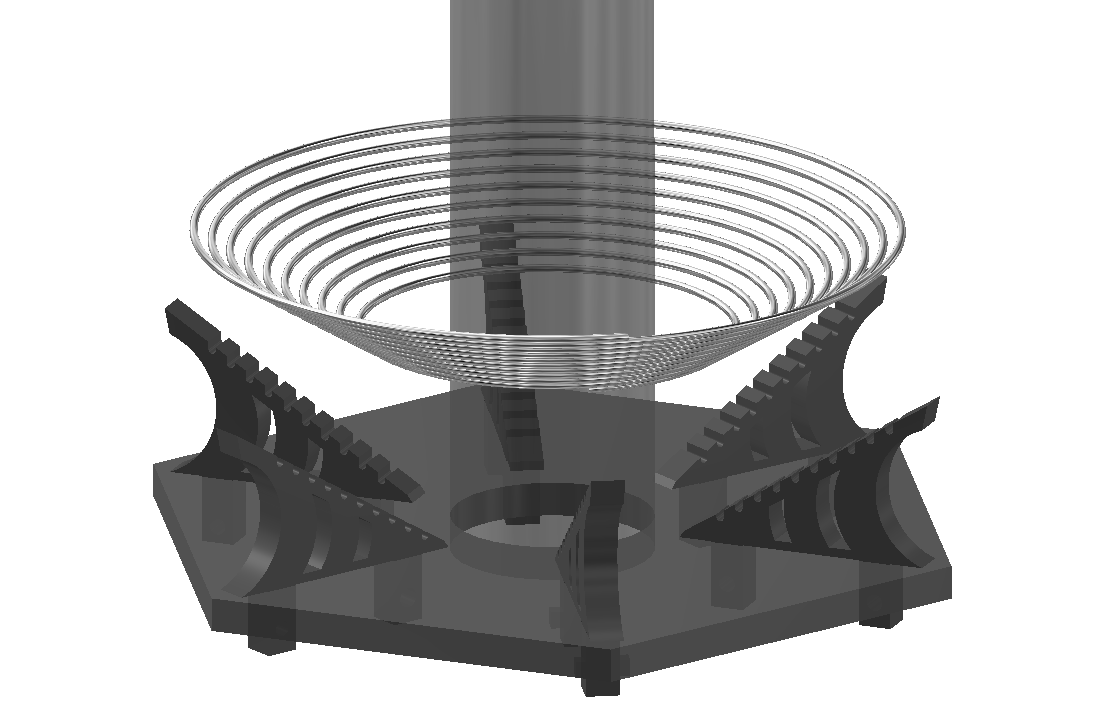
\includegraphics[width=1\textwidth]{kassandra/resources/endeMeinerHoffnung.png}
    \caption{3D view of the primary supports}
    \label{fig:primary-supports}
\end{figure}

To avoid gluing the supports to the base plate, a bolt was used as shown in figure \ref{fig:stayer} to keep it in place. This mechanism was mostly designed for testing purposes as it is easier to assemble and disassemble. In a possible future version or commercial release it would be safer if the supports were glued on. Also as shown the supports have a unique design. This was mostly done, to make them look more elegant and not stand out too much. That makes them lighter, but given that the supports are just a small fraction of the tesla coil's weight, it doesn't make much of a difference.

\begin{figure}[h!]
    \begin{subfigure}{0.5\textwidth}
        \centering
        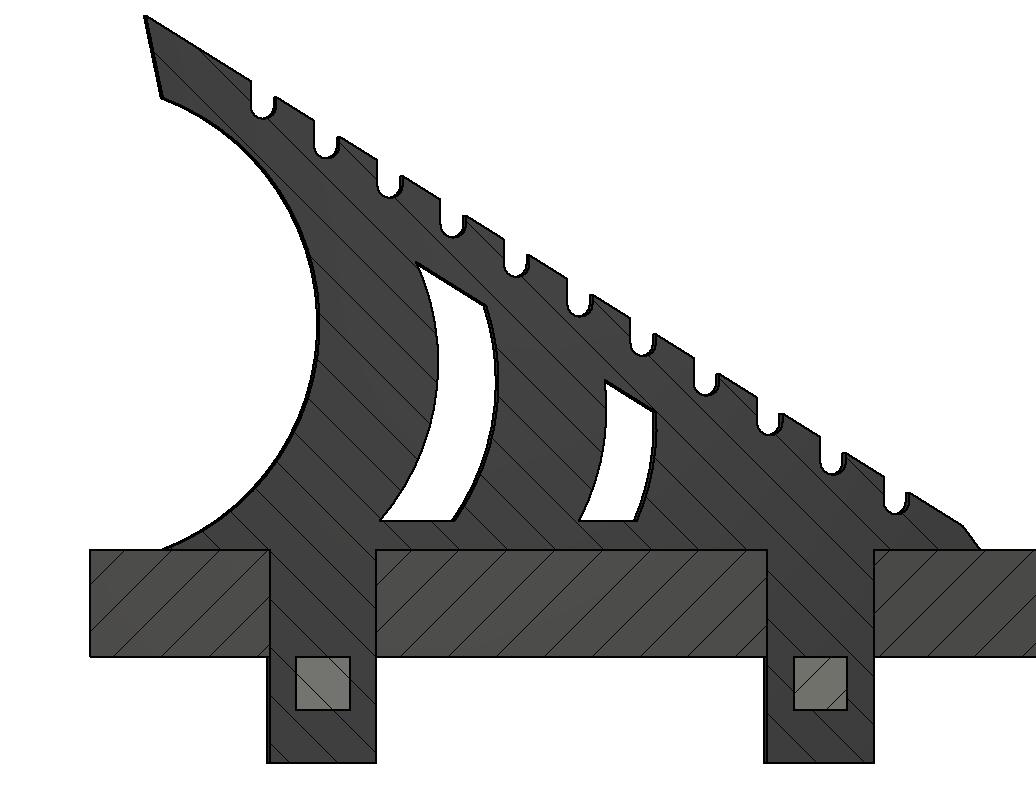
\includegraphics[width=\textwidth]{kassandra/resources/endeMeinerHoffnungInSemi2DStayer.PNG}
    \end{subfigure}%
    \begin{subfigure}{0.5\textwidth}
        \centering
        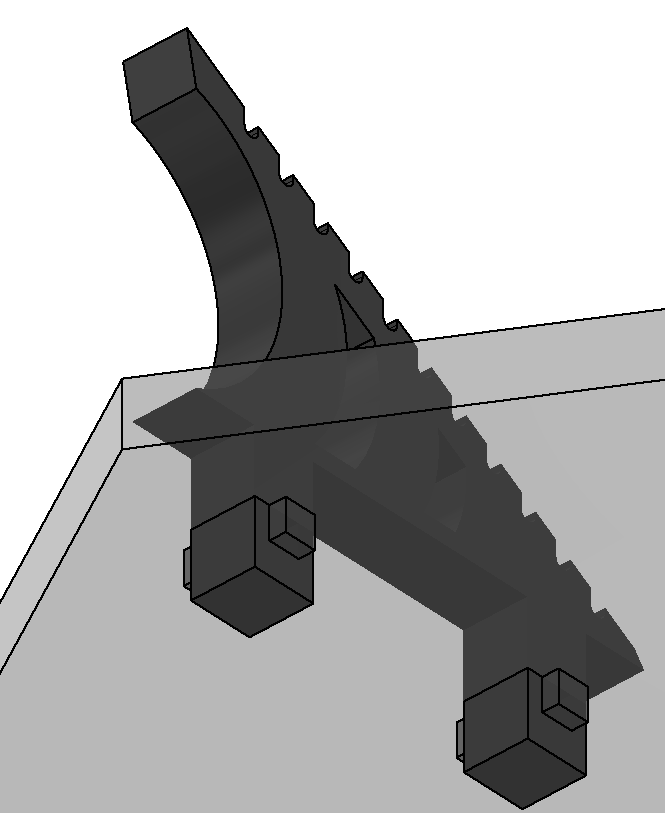
\includegraphics[width=0.7\textwidth]{kassandra/resources/endeMeinerHoffnungIn3DStayer.PNG}
    \end{subfigure}
    \centering
    \caption{Fastening of the supports}
    \label{fig:stayer}
\end{figure}

\subsection{Secondary Coil}

The core of the secondary coil was one of the easier parts to design, because it essentially just consists of a 30mm \gls{pmma} tube with a thickness of 3mm. A few millimeters from the top of the tube, a small hole was drilled to bring the wire to the inside and connect it to the top electrode. The 330 turns of 0.35mm wire were then wound by hand and then coated with protective and insulating vanish to prevent the wire from loosening and cross-arcing to occur.

\todo{Das Gerüst für die zwei spulen. Stayer Desgin und funktion.}

\section{Top Electrode}

Technically the tesla coil would also work without a top electrode by simply using the end of the secondary coil's wire as the arcing point. But given that the wire of the secondary has a small diameter and is made of copper it would likely melt or at least start to deform, when it emits a spark. To ensure the arcing point stays in tact the wire is connected to another material - in this case it's a welding electrode made of a tungsten alloy. 

The holder, that keeps the electrode at the top of the coil is made of two parts. The first as seen in figure \ref{fig:top-electrode} are two copper pieces that are kept together with a thread and in between the wire of the secondary is clamped. There are also two notches on each to enable fastening and opening with a flat wrench. To mount the tungsten electrode, a small fit was drilled into the top surface of the copper piece. 

The second part is a \gls{pmma} piece with another fit a the top this time for the copper piece. On one side there is also a gap to direct the wire of the secondary to the inner part. 

\begin{marginfigure}[-8cm]
    \centering
    \includegraphics[width=0.7\textwidth]{kassandra/resources/endeMeinerHoffnungFürBlitz.PNG}
    \caption{Mounting of the top electrode}
    \label{fig:top-electrode}
\end{marginfigure}

\subsection{It's not a Bug, it's a Feature}

Because the tesla coil driver was very underdimensioned, the plasma flame forming on the top electrode was very small and often had to be ignited and stabilized by another conductor held close to it. This was realized by placing a second, ancillary electrode over to main electrode. This ancillary electrode is held by a conapy-like structure, resting on three \gls{pmma} rods. It was press fitted into a flat copper cylinder, which was loosely screwed into the cap. This way its height, and therefore the gap between the two electrodes could be changed by turning the ancillary electrode. 

\begin{marginfigure}[-3cm]
    \centering
    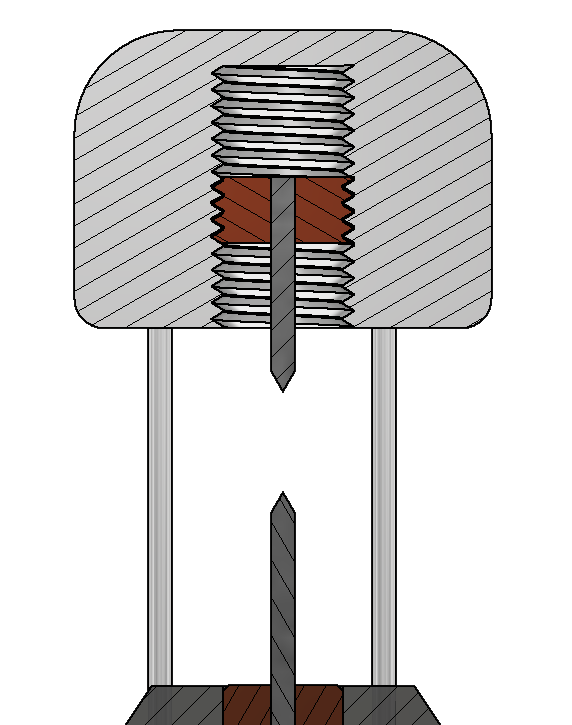
\includegraphics[width=\textwidth]{kassandra/resources/mirGehtsSuperDanke.png}
    \caption{Mounting of the ancillary electrode}
    \label{fig:ancillary-electrode}
\end{marginfigure}

To further examine the effect of the material of the cap, three different versions have been made. One out of \gls{pmma}, and two out of Aluminium, one of which is as smooth as possible and one as pointy as possible.

\begin{figure}
    \centering
    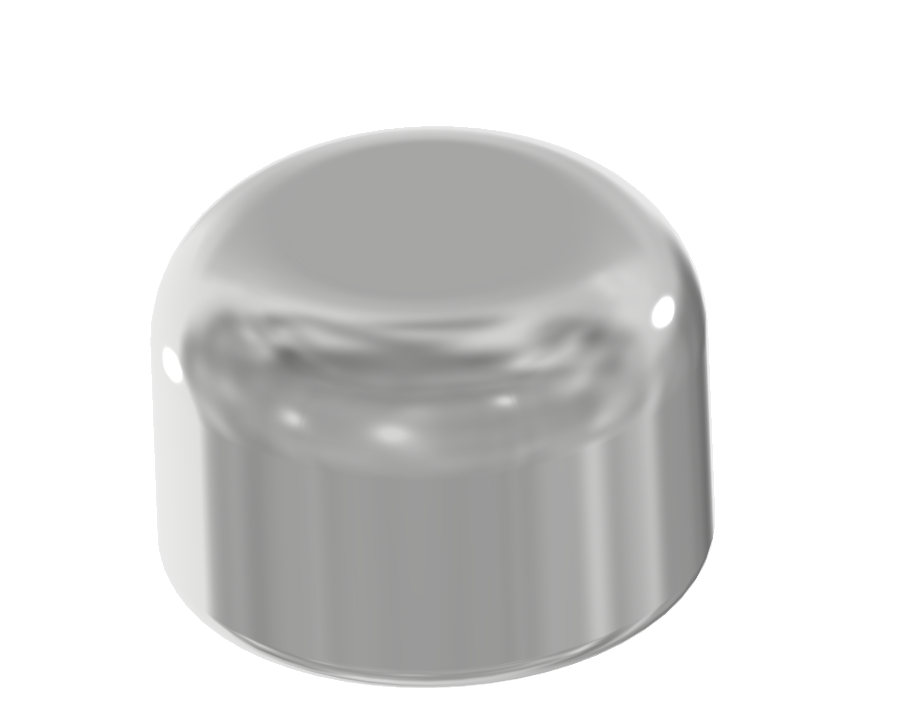
\includegraphics[width=0.3\textwidth]{kassandra/resources/mirGehtsSuperDankeSmooth.png}
    \caption{Smooth Cap}
    \label{fig:smooth-holder}
\end{figure}

\begin{figure}
    \centering
    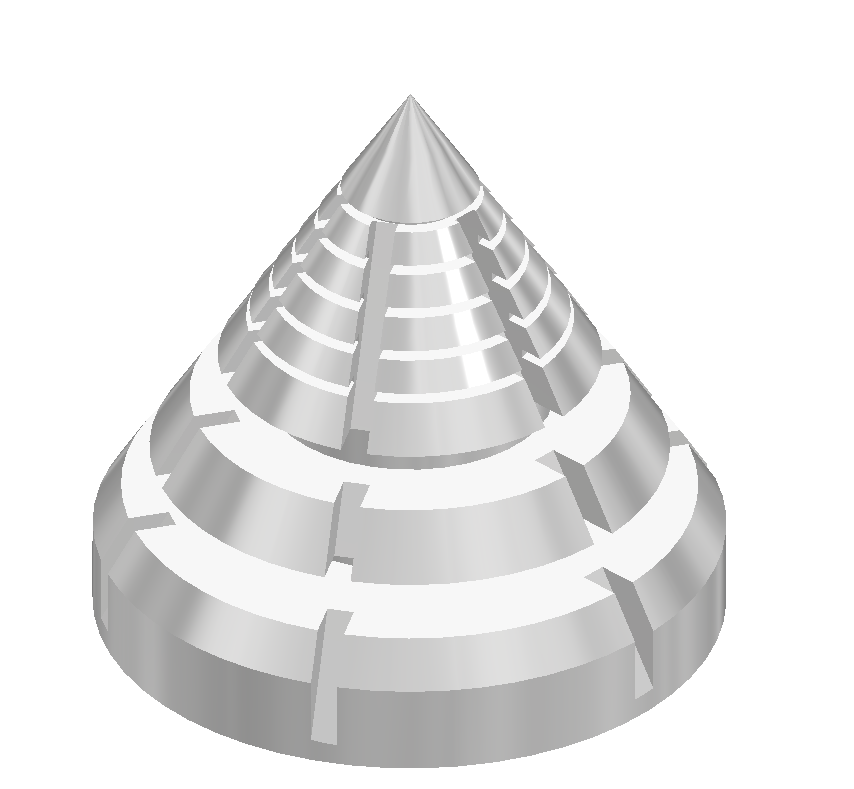
\includegraphics[width=0.3\textwidth]{kassandra/resources/mirGehtsSuperDankeEdgy.png}
    \caption{Pointy Cap}
    \label{fig:edgy-holder}
\end{figure}

ok i gebs auf

\section{PCB Enclosure}

\todo{warum hexgon? - looks nice - no}